%#!platex -kanji=utf8 hb.tex
\chapter{画像の張り込み}
% これはただのダミーテキスト.
% 文字コードを判定するための意味のない文字列.
% これくらい記述すれば大丈夫かな.
% Emacs のくせに生意気な.
% Emacs の分際で自動判別とか.
% Mac OS X のテキストエディッタの文字コード自動判別はうまくいかないぞ.

\section{図に関する制約と画像の扱い}\label{sec:figure}

図の挿入に関しては大きく分けて2通りの方法があります.一つはペイントソ
フトなどで書いた画像をそのまま取り込む方法, もう一つは{\LaTeX}の
\env{picture}環境で図を直接書く方法です.

%\LaTeX には\Env{picture}環境と呼ばれる簡単な\Z{作図}をするための
%描画環境が用意されています.この\Env{picture}環境を拡張した
%\Y{epic}, \Y{eepic}, \Y{pict2e}などが存在し,ある程度の作図が
%できるコマンドが用意されています.\Env{picture}環境とその周辺の詳しい
%事は\wasyo{\COMP}\cite{latexcomp}や\wasyo{\GCOMP}\cite{graphicscomp}
%を参照してください.

何らかの外部プログラムで作成した BMP, JPEG, PNG, EPS, PDF 等の画像を
\LaTeX に張り込むためには,一般的には\sty{graphicx}パッケージを用います.

\LaTeX 自身では画像ファイルを直接的に扱う仕組みは用意されておらず,
画像ファイルに関する多くの処理をデバイスドライバという外部プログラムに依
存した形を取るため,自分の使おうとしているデバイスドライバがどのような画
像処理に対応しているのかを知ってください.最終的に出力したい文書形式が
PDFならば{dvipdfmx},\PS ならば{dvips}を使う事になります.
近年ではDVI 形式から直接 PDF を生成できるdvipdfmx を使う事を強く推奨し
ます.dvipdfmx を用いる事でBMP, JPEG, PNG, \Z{EPDF}(単一ページのPDF), 
EPS 画像の張り込みが可能となり,さらに DVI ファイルから直接 PDF を生成す
る事ができます.

最近の動向として論文等の提出,印刷には PDF を用いる場合が増えている
ようです.dvipdfmx を使えば \LaTeX でそのまま PDF 画像の埋め込み
等もサポートしているため,今後は何かしらの問題がない限り,dvipdfmx 
を使うようにすると何かと便利だと思われます.
\zindind{画像}{の張り込み}%

近年まで{\LaTeX}ではEPS以外の画像の張り込みは難しいという都市伝説的な定
説がありましたが,現在は dvipdfmx の登場により状況は幾分変化しています
し,これからも変化すると考えられます.



\section{画像ファイルの張り込み}\seclab{gazou}

\LaTeX\ ではビットマップ画像や,曲線の描画などの多くの処理をデバイスドラ
イバと呼ばれる外部のプログラムに依存しています.そのため,\LaTeX\ で画像
ファイルを扱う場合は,まずデバイスドライバを用途別に選択する事になりま
す.


\subsection{デバイスドライバの選択}

%各種のデバイスドライバプログラムにおける画像形式に対する対応状況を
%\tabref{ddimage}に示します(\genzai での対応状況).
\begin{table}[htbp]
 \begin{center}
  \caption{各種デバイスドライバの画像形式対応状況}\tablab{ddimage}
  \begin{tabular}{ll}
  \TR
  \Th{デバイスドライバ} & \multicolumn{1}{c}{\Th{対応画像形式}}\\
  \MR
  xdvi      & EPS*  \\
  dvips     & EPS   \\
  dvipdfmx & EPS*, EPDF, PNG, BMP, JPEG\\
  \Dviout    & EPS*, {Susie} {plug-in} により他の形式に対応可能\\
  \BR
  \end{tabular}
 \end{center}
\end{table}
星印がついているものは\GS などの外部プログラムを必要とする形式です.

{\LaTeX}で画像を張り込む時,多くの場合は標準的に\sty{graphicx}パッケージを
使う事になります.dvipdfmx を使っている場合はパッケージオプション
を\Option{dvipdfmx}とします.

\begin{intext}
\usepackage[dvipdfmx]{graphicx}
\end{intext}

これにより\sty{graphicx}パッケージは\fl{dvipdfmx.def}という設定ファイルを
読み込みます.もしも \Fl{dvipdfmx.def}というファイルが存在しないようであ
れば,以下のURLからファイルを取得し`\str{$texmf/tex/latex/graphics/}'等
のディレクトリにコピーしてください%
\footnote{\url{http://tex.dante.jp/jou1/dvipdfmx.def}}.


古い \TeX/\LaTeX (2006年以前)がインストールされているのであれば,
\option{dvipdfmx}ではなく,\Option{dvipdfm}オプションを指定して,
dvipdfmx で PDF をデバイスドライバとします\footnote{何かしらの
理由がない限り \TeX 環境は定期的に更新する事が望ましいです.}.

\begin{intext}
 \usepackage[dvipdfm]{graphicx}
\end{intext}

Unix系OSならば{\PS}のほうが良いでしょうから\Option{dvips}を\sty{graphicx}
パッケージのオプションとします.{dvipsk}であろうが{pdvips}だろ
うが\Option{dvips}オプションを使います.

他には{xdvi}や,Windows であれば \Dviout も指定できます.
Windowsの方で手持ちの画像のほとんどがビットマップで存在するならば\Dviout
をデバイスドライバに選択すれば良いでしょう.\Dviout ではプレビューも印刷も
行えます.
\Dviout の場合は\Dviout がインストールされているフォルダの
\fl{GRAPHIC/LATEX2E/dviout.def}というファイル
を \fl{\$texmf/tex/latex/graphics/} にコピーしてください\footnote{\Dviout の
場合EPS画像を取り込むときは{\GS}にてEPSを\Z{PPM}に変換してから画像
を表示しますから{\Dviout}の{Ghostscript}に関する設定を適切に行っ
てください.}.

EPS画像が多いならばいずれにしても1度EPSからPDFに変換してから
{dvipdfmx}を使うのが良いと思われます.%\unixos ならば手持ちの画像を
%EPSに変換して{dvips}を使うことになるでしょう.


\subsection{具体的な手順}

画像ファイルを\LaTeX の文書に張り込むには,一般的に次のような手順を踏む
事になります.

\begin{enumerate}
\zindind{フォント}{のアウトライン化}%
\zindind{PDF}{画像の張り込み}%
\item 外部プログラムでPDFやEPS形式でファイルを保存.保存する時の
      オプションで可能であればフォントはアウトライン化し,カラーに
      依存しないようなファイルとします.
\item 文書のプリアンブルで\sty{graphicx}パッケージを使う事を宣言します.
\item \sty{graphicx}パッケージには\K{デバイスドライバ}を指定します.
      \PS 形式の文書を出力するならば,\Option{dvips}を指定します.PDFを作成し
      たいときは{dvipdfmx}を使うために\Option{dvipdfmx}を指定します.
\item EPS以外の画像であれば\LaTeX が解釈できる形で\K{バウンディングボッ
      クス}を指定します.
\item  図を挿入すべき場所に \C{includegraphics}命令を使ってファイル名を
      示します.
\end{enumerate}

デバイスドライバのdvipdfmx 等は画像ファイルを扱う事が可能ですが,\LaTeX
は画像ファイルを直接扱う事ができず,画像に関する情報を取得できません.
そのため,dvipdfmx において\Z{JPEG},\Z{PNG},\Z{PDF}, \Z{BMP}の画
像ファイルは\KY{バウンディングボックス}という画像の(\Z{原点座標}を含む)
\zindind{画像}{の原点座標}%
サイズ情報を与える事で張り込む事が可能です.一般的には画像の横の長さと縦
の長さのサイズを指定する事となります.バウンディングボックスは
\Va{filename}{img}という画像ファイルがあれば,\Va{filename}{bb}という
ファイルを\sty{graphicx}パッケージが参照するようになっています.

\Dvipdfm に付属する{ebb}というプログラムで画像のバウンディングボッ
クス情報のファイル \Va{filenam}{bb}を作成できます.対応している画像形式
はJPEG, PNG, PDF です\footnote{ebb以外にも{identify}コマンドや{file}コ%
マンドでサイズ情報は知る事ができますし,WindowsやMac~OS~Xであれば%
{エクスプローラ}や{ファインダー}にも表示されます.}.

JPEG,PNG,PDF,EPSを直接PDFに張り込めます.具体的な手順として
は,ファイルの存在するディレクトリで
%\begin{InTerm}
%\type{ebb filename.jpg}
%\end{InTerm}
とすれば拡張子が\exten{bb}の\Va{filename}{bb}というファイルが
作成されます.作成された\Va{filename}{bb}を見てみます.

\begin{intext}
%%Title: ./filename.jpg
%%Creator: ebb Version 0.5.2
%%BoundingBox: 0 0 595 842
%%CreationDate: Tue Dec 30 13:04:10 2003
\end{intext}

上記のように\va{ファイル名},\va{作成プログラム}, \va{バウンディングボッ
クス}, \va{作成日時}の情報が出力されます.沢山\Va{filename}{bb}のファイ
ルを保存しておくのが好ましくない場合は,該当する画像ファイルを読み込んで
いる箇所で,次のようにすれば\Va{filename}{bb}がなくても良い事になりま
す.

\begin{intext}
\includegraphics[bb={0 0 595 842}]{filename.jpg}
\end{intext}

使用する画像のファイル名の\Va{ファイル名}{拡張子}は
\qu{\fl{filename.png}}のように\Va{8文字}{3文字}としたほうが互換性の上で安
全です.


\begin{Exe}
仮にファイル名が\fl{image.png}の画像があったとすれば,コンソールから
\type{ebb image.png}として\fl{image.png}用の\fl{image.bb}が作成される事
を確認してください.この\texttt{image.bb}は画像ファイルの縦横を正しく扱
うためのファイルです.\texttt{image.bb} を見れば分かりますが,中身は次
のようなものになっていると思います.

\begin{intext}
%%Title: ./image.png
%%Creator: ebb Version 0.5.2
%%BoundingBox: 0 0 595 841
\end{intext}

\qu{\str{BoundingBox}}とは原点座標と画像の縦横の長さの値です.次にソース
ファイルを以下のようにします.

\begin{intext}
\documentclass[papersize]{jsarticle}
\usepackage[dvipdfmx]{graphicx}
\begin{document}
\centering \includegraphics[width=4cm]{image.png}
\end{document}
\end{intext}

後はいつも通りにタイプセットしてDVIファイルを生成し{dvipdfmx}でPDF
を作成します.これにより \fl{image.png}が張り込まれた PDF が生成されるは
ずです.
\end{Exe}

\subsection{張り込みにおけるオプション}

外部プログラムで作成して,すでに存在するような画像は \C{includegraphics}
命令で張り込みます.
\begin{usage}
\includegraphics[$\<設定>$]{$\<ファイル名>$} 
\end{usage}
%\begin{Syntax}
%\C{includegraphics}\opa{設定}\pa{ファイル名}
%\end{Syntax}

\val{設定}に関しては以下に示すようなオプションが使用できます.

\begin{description}
\zindind{画像}{の高さ}%
 \item[\str{height=}\val{高さ}]
    単位付きで画像の高さを指定します.
 \item[\str{totalheight=}\val{総合的な高さ}]
    単位付きで画像の総合的な高さを指定します.
\zindind{画像}{の幅}%
 \item[\str{width=}\val{幅}]\indindz{幅}{画像の}%
    単位付きで画像の幅を指定します. 
 \item[\str{scale=}\val{数値}]
\zindind{画像}{の拡大}%
    画像の拡大率を指定します. \indindz{拡大}{図の}
 \item[\str{angle=}\val{角度}]
\zindind{画像}{の回転}%
    {反時計回りに}画像を回転する角度を指定します. 
 \item[\str{origin=}\val{原点}]
    画像の基準点を決めます. 
 \item[\str{bb=}\val{領域情報}]
    \KY{バウンディングボックス}と呼ばれる画像の大きさと原点座標を指定します.
    画像のどの領域を使うべきかを指定します.\zindind{画像}{のバウンディングボックス}%
    \qu{\str{bb=0 0 640 480}}とすると原点を
    \xy{0}{0}として縦横\qu{$640\times480$}
    の領域を使うようにします.
 \item[\str{viewport=}\val{領域情報}] 
\zindind{画像}{の切り抜き}%
	    画像の利用領域を指定します.切り抜きです.
%	    \str{viewport={30 30 600 40}}
 \item[\str{trim=}\val{領域情報}] 
\zindind{画像}{のトリミング}%
	    画像の端を切り抜きます.
%	    \str{trim={3 3 2 2}}
 \item[\str{noclip}] 
  画像用に使うべき領域を元の画像がはみ出している
  場合に画像を切り抜かないようにします.
 \item[\str{clip}] 
\zindind{画像}{のクリッピング}%
  画像が確保された領域よりも大きい場合は
  切り抜きします.
 \item[\str{draft}] 
 実際に画像を張り込まずに画像が占有す
 るだろう領域が枠による代替表示になり,ファイル名を表示します.
 \item[\str{keepaspectratio}] 
\zindind{画像}{の縦横比}%
 拡大縮小したときに縦横比を保存するようにします.
 \sty{graphicx}パッケージの標準では保存されます.
\end{description}

\begin{Exe}
ご自分の持っている画像\val{ファイル}を\val{デバイス}が
取り込めるのかを試してみください(行頭のパーセントは取り除き,
\fl{images}フォルダに\Fl{gnu-head.pdf}と\fl{gnu-head.bb}があると仮定します).
\begin{inout}
\usepackage[dvipdfmx]{graphicx}
\includegraphics[width=3cm]
  {gnu-head}
\end{inout} 
\end{Exe}

\begin{inout}
\usepackage[dvipdfmx]{graphicx}
\includegraphics[width=2cm,
  trim=20 20 20 20]
  {gnu-head} 
\end{inout}

\begin{inout}
\usepackage[dvipdfmx]{graphicx}
\includegraphics[width=2cm,
  clip,viewport=131 304 459 548]
  {gnu-head}  
\end{inout}

\begin{inout}
\usepackage[dvipdfmx]{graphicx}
\includegraphics[width=2cm,angle=30,
  clip,viewport=131 304 459 548]
  {gnu-head}   
\end{inout}

\begin{inout}
\usepackage[dvipdfmx]{graphicx}
\includegraphics[width=2cm,angle=90,
  clip,viewport=131 304 459 548]
  {gnu-head}    
\end{inout}

\subsection{画像の拡大や回転等の操作}

図などを反時計回りに\kaku{90}回転させる事があるでしょう.
その場合は \Cmd{rotatebox}命令を使います.
\begin{usage}
\rotatebox[$\<設定>$]{$\<回転角度>$}{$\<要素>$}
\end{usage}
%\begin{Syntax}
%\Cmd{rotatebox}\opa{設定}\pa{角度}\pa{要素}
%\end{Syntax}
これは \cmd{includegraphics}の任意引数に
\qu{\str{angle}}を使った事と同じです.
 \cmd{rotatebox}は図に限らずあらゆる要素(表も可能)を
\Z{回転}します.\val{設定}の項目には以下のような
ものがあります.
\begin{description}
\item[\str{origin=}\val{ラベル}] 
 要素を回転するための原点を指定します.%%
 左\qu{\str l},右\qu{\str r},中央\qu{\str c},
 上部\qu{\str t},下部\qu{\str b}が指定できます.
\item[\str{x=}\val{長さ}] 
$x$方向の原点の位置を直接\val{長さ}を指定します.
\item[\str{y=}\val{長さ}]
$y$方向の原点の位置を直接\val{長さ}を指定します.
\end{description}

\indindz{回転}{文字列の}%%%
\begin{inout}
\rotatebox{70}{文字列など}の
\rotatebox[origin=c]{60}{回転とか}は
\rotatebox[origin=b]{50}{どう}
\rotatebox{30}{ですか?}
\end{inout}
%
要素を\K{拡大縮小}するには \cmd{scalebox}を
使います.\index{拡大}\index{縮小}\indindz{拡大}{文字列の}
\begin{usage}
\scalebox{$\<横方向の拡大率>$}[$\<縦方向の拡大率>$]{$\<要素>$}
\end{usage}
%\begin{Syntax}
%\Cmd{scalebox}\pa{横の拡大率}\opa{縦の拡大率}\pa{要素}
%\end{Syntax}
\val{拡大率}には長さを指定します.\begin{inout}
\scalebox{2.3}{拡大縮小}\par
\scalebox{3}[1]{拡大縮小}
\end{inout}

要素の\K{反転}には \cmd{reflectbox}を使います.
\begin{usage}
\reflectbox{$\<要素>$} 
\end{usage}
%\begin{Syntax}
%\Cmd{reflectbox}\pa{要素}
%\end{Syntax}
\begin{inout}
\reflectbox{文字列の反転}\par
\reflectbox{山は山}\par
\scalebox{-1}[1]{これも反転}
\end{inout}

リサイズには \cmd{resizebox}を使います.
\begin{usage}
\resizebox{$\<幅>$}{$\<高さ>$}{$\<要素>$}
\end{usage}
%\begin{Syntax}
%\Cmd{resizebox}\pa{幅}\pa{高さ}\pa{要素}
%\end{Syntax}
要素のリサイズ後の幅を\val{幅}に,高さを\val{高さ}にします.
どちらか一方の拡大・縮小率に合わせたいときは\qu{\str!}を
使います.
\begin{inout}
\resizebox{!}{1cm}{リサイズ}\par
\resizebox{3cm}{!}{リサイズ}
\end{inout}

以上の \cmd{rotatebox}, \cmd{scalebox}, \cmd{reflectbox},
 \cmd{resizebox}は文字列,表,図,\env{minipage}環境など
の段落などにも使えます.\indindz{回転}{表の}%%
\begin{inout}
\newcommand{\testtab}{%
\begin{tabular}{|c|}
 \hline \LaTeX\\ \LaTeXe \\ \hline
\end{tabular}}
\rotatebox{80}{\testtab}~
\reflectbox{\testtab}
\end{inout}

\subsection{dvipdfmx におけるEPS画像の扱い}

dvipdfmx の場合は基本的にPDF,JPEG,PNG,BMP,MetaPost 形式の
画像しかサポートしておりませんので,EPS形式の画像は何らかの形でPDFに変換
してから取り込む事になります.\LaTeX の原稿中で \C{includegraphics}命
令を用いてEPS画像を張り込んでいる場合は,dvipdfmx が DVI から PDF への
変換の段階で \GS プログラムを毎回実行してEPSをEPDFに変換しています.
そのため,dvipdfmx をデバイスドライバとして使用しているときには極力
EPSではなく,EPDF画像を張り込むようにします.外部プログラムがPDFでの
保存に対応していないようであれば,あらかじめEPSをEPDFに変換すると
処理速度の向上につながります.

このEPSファイルは{Ghostscript}の\qu{pdfwrite}というデバイスを使って
変換する事がほとんどです.その時に
{epstopdf}か{ps2pdf}などを使います\footnote{Vine Linux の場
合は{ps2jpdf}という日本語フォントを埋め込まない PDF を作成できる
プログラムもあります.\type{apt-get update; apt-get install ps2jpdf}
でインストールできます.}.
{epstopdf}はPDFにEPSの{\BB}を反映してくれます.
%{ps2pdf}系を使う場合はPDFに{\BB}がうまく反映されません(\genzai).
%以下のようなシェルスクリプト\fl{eps2pdfs}を作成します.

\begin{intext}
#!/bin/bash
EPS=`ls *.eps`;
for fig in $EPS; do
   epstopdf $fig
   $f=`basename $fig .eps`
   grep "^%%BoundingBox:" $fig > $f.bb
done
\end{intext}

\fl{eps2pdfs}を\Z{PATH}の通っている場所(\fl{/usr/local/bin/} など)に複
製したならば
%\begin{InTerm}
%\type{eps2pdfs}
%\end{InTerm}
とすると同ディレクトリのEPSファイルが全てPDFに
変換されます.\val{file}{eps}があったとすればこれは
\val{file}{pdf}と\val{file}{bb}が作成されます.


\subsection{PDF画像の切り抜きと\BB}

%しかし,昨今はEPSではなく,直接PDFしか存在しない場合があり,
%割と \BB を正しく扱えるプログラムというのも少ないようで
%あまり多くはないようだ.%コマンドラインから人が目で見て計測する
何かしらのプログラムで作成したPDFには余計な余白が含まれている
事がしばしばあります.これを自動的に切り抜く方法の一つとして
\Person{Heiko}{Oberdiek}による {pdfcrop} を使う事により,
PDF画像の余白の切り抜きを行う事ができます(要 \PDFTeX, Perl, \GS).
使い方はコンソールから次のようにするだけです.
%\begin{InTerm}
% \type{pdfcrop input.pdf}
%\end{InTerm}
これにより \fl{input-crop.pdf}が生成されます.

また,PDFの正確な\BB を取得する一つの方法として
{pdfinfo} を使う事が考えられます.

{pdfinfo} によって表示される情報は以下のような構成になっています.

%\begin{OutTerm}
%Creator:        TeX
%Producer:       pdfTeX-1.10b
%CreationDate:   Sat Apr 15 21:23:00 2006
%Tagged:         no
%Pages:          1
%Encrypted:      no
%Page size:      416 x 40 pts
%File size:      7995 bytes
%Optimized:      no
%PDF version:    1.4
%\end{OutTerm}

{pdfcrop} によって切り抜きを行った画像であれば,
`\str{Page size: 416 x 40 pts}'を適切に加工すれば\BB と
して使えるようになるでしょう.%`\str{PDF version}'が`1.4'であるため
%{ebb}では失敗するでしょう.

以下のようなスクリプト \Fl{makebb}を用意します\footnote{\url{http://tex.dante.jp/jou1/makebb}}.

%\begin{plainfile}
%#!/bin/sh
%# 引数として与えられたディレクトリを作業対象とする
%cd $1;
%# PNG 画像の BoudingBox の生成を ebb により行う
%for f in `ls *.png`; do 
%   if [ -f `basename $f .png`.bb ] ; then 
%      echo "already `basename $f .png`.bb exits."
%   else 
%      ebb -v $f; 
%   fi
%done
%# JPEG 画像の BoundingBox の生成を ebb により行う
%for f in `ls *.jpg`; do 
%   if [ -f `basename $f .jpg`.bb ] ; then 
%      echo "already `basename $f .jpg`.bb exits."
%   else 
%      ebb -v $f; 
%   fi
%done
%# PDF 画像の BoundingBox の生成を pdfinfo によって 行う
%for f in `ls *.pdf`; do 
%   if [ -f `basename $f .pdf`.bb ] ; then 
%      echo "already `basename $f .pdf`.bb exits."
%   else 
%      echo "creating `basename $f.pdf`.bb..."
%      pdfinfo $f | grep -e 'Page size:' | \
%      sed -e 's/x//; s/Page size:/\%\%BoundingBox: 0 0 /; s/pts//;' \
%      > `basename $f .pdf`.bb
%   fi
%done
%\end{plainfile}

これを例えば,適当にアクセス権を与えて \type{makebb img}
とすれば,\fl{img}ディレクトリに存在するPNG, JPEG, PDF画像の
\BB を作成します.

\Z{ストリームエディッタ}の{sed}がない場合は適当に 
{Perl}等で実行してください.

%このようにしてEPSからPDFに変換したファイルは
%{\LaTeX}の原稿で次のように取り込むことができます
%(行頭のパーセントは取り除いてください).
%\begin{inout}
%\usepackage[dvipdfmx]{graphicx}
% \includegraphics[width=3cm]
%    {images/gnu-head}
%\end{inout}

\subsection{dvipsと{dvipdfmx}の併用}

dvipskとdvipdfmx の両方を併用している(
\Z{Unix系OS}の方で普段は\PS で印刷していて,
提出用にPDFを作成するなど)場合は\fl{images}ディレクトリ
を作成し,そこに\val{image}{eps},\val{image}{pdf},
\val{images}{bb}の三つのファイルを置きます.次に
原稿中で次のように \C{includegraphics} 命令を使うとき
{拡張子を省略します}.

\begin{intext}
\includegraphics[width=3cm]{images/gnu-head}
\end{intext}

すると\sty{graphicx}パッケージに渡されたパッケージオプションに
従って,張り込まれる画像の優先順位が変わりますので,
\Option{dvips}を指定している場合はEPSが,\Option{dvipdfmx}を
指定している場合はPDFが張り込まれるようになります.
次のように\sty{graphicx}の読み込みの仕方を変更するだけです.

\begin{intext}
%\usepackage[dvips]{graphicx}  % dvipsk   の場合
\usepackage[dvipdfmx]{graphicx} % Dvipdfmx の場合
\end{intext}


\subsection{レポート・論文における図の張り込み}

レポートや論文などで図には\K{図見出し}を付けて\K{中央揃え}に
するのが望ましいと思われますので,次のように使う事になります.

\begin{intext}
\begin{figure}[htbp]
 \begin{center}
   \includegraphics[width=10cm]{images/file.eps}
   \caption{図見出し}\label{fig:samplefig}
 \end{center} 
\end{figure} 
\end{intext}

ただし,これを毎回
書くのは面倒なので次のような図用の\env{myfig}命令を
作成します.

\begin{intext}
\newcommand{myfig}[4][width=.8\linewidth]{%
\begin{figure}[htbp]%
   \centering\includegraphics[#1]{#2}%
   \caption{#3}\label{fig:#4}%
\end{figure}}
\end{intext}

このように定義しておけば次のように簡単に使えます.

\begin{intext}
以上の考察から図~\ref{fig:sample}のような図が得られる.
\myfig[width=100pt,clip]{images/file.eps}{図の張り込みの例}{sample}
\end{intext}

浮動体の図はDVIファイルに出力されるときに思いもよらない場所まで旅をしま
すので,思い通りの場所に図が配置されなくても腹を立てないでください.
そもそも図表に対して\yo{上記の図は何々}とか\yo{下記の図は何々}という表現
は間違いで,全ての図表は\yo{図~3.1は何々}のように番号で参照します.です
から本来は図表がどのような場所に旅立っても困らないはずです.

%HOGE 1037 例題を作成する

\subsection{汎用的な画像の作成と活用}\seclab{excel:kowaza}

\LaTeX とdvipdfmx を用いる事で,JPEG, PNG, BMP, EPS, PDF 等の画像を張り
込む事が可能でした.しかし,外部プログラムによってはそれらの形式の画像ファ
イルの\Z{書き出し}(変換)に対応していない場合があります.この場合はある
特定のプログラムから,\Z{仮想プリンタ}に対して画像の内容を送信し,EPSか
PDFで保存するのが手短にできる方法となります.

Windows であれば {PrimoPDF}等のフリーの変換プログラムがあります.
Mac~OS~XであればOSそのものがPDFでの書き出しに対応しています.%\unixos では

現在お使いの環境に{Adobe Acrobat}がある場合は,Acrobatを活用し
ていただいて構いません.

\subsection{プログラム特有の処理}\seclab{picture:program}

特定の外部プログラムからグラフや画像を取り込むときには幾つかコツが必
要です.\secref{excel:kowaza}での張り込み方が他のアプリケーション
でも適用できる場合が多いので,上記の方法を試してみてください.

どのプログラムを使用していても最終的に出力したい画像のサイズを元のプログ
ラム側で調節してから{\LaTeX}に張り込むようにすると問題も少ないでしょう.
\sty{graphicx}パッケージの拡大縮小を使うと印刷品質が落ちます.各プロ
グラムにおける設定方法は以下の通りです\footnote{プログラムのバージョンに
よっては幾分操作方法が異なると思います.}.

\begin{description}
\item[{Illustrator}]
  可能であれば文字はアウトライン化します.
  Adobe PDF の互換性では \win{Acrobat 4 (PDF 1.3)}を指定する
  ようにすると,問題が発生しづらいと思われます.
  ツールバーの\win{別名で保存}でファイル形式を\qu{Adobe 
  PDF}として保存します.PDF形式での保存オプションで\yo{サムネー
  ルを埋め込み}の{チェックを外して},\yo{圧縮}はしないように
  してください.{Illustrator}の場合は用紙サイズが切り抜かれ
  ませんので何らかの方法({Adobe Acrobat}や \cmd{includegraphics}
  命令の \option{trim} オプション)で切り抜きを行う必要があります.
\item[{Photoshop}]
  \win{ファイル},\win{複製を保存}を選び\yo{保存形式}
  を\qu{Photoshop PDF}にして保存します.ビットマップ画像は圧縮しないほうが印
  刷品質が良いようです.
\item[Gnuplot] フリーのプロットソフトで \PS, \Y{PSTricks}, {Tgif},
  {Illustrator}, \Y{eepic}, [MetaFont]{\MF},
  [MetaPost]{\MP}等,多くの形式で画像の書き出しをサポートしています.
  {Octave}も{MATLAB}類似でGPLの数値演算ソフトで Gnuplot をもとに
  開発されていますので手順は Gnuplot の場合とほとんど同じです.\Y{eepic}
  パッケージで対処するには,例えば Gnuplot 側で次のようにします.

\begin{intext}
set output 'plotfile1.tex'\\
set term eepic rotated dashed\\
plot x
\end{intext}

すると,カレントディレクトリに\fl{plotfile1.tex}が作成されますから,
\Y{eepic}パッケージ等を用いて,\LaTeX の原稿側で次のように記述します.

\begin{intext}
\documentclass[dvipdfmx]{jsarticle}
\usepackage{graphicx,color,epic,eepic,amssymb}
\begin{document}
\input{plotfile1}
\end{document}
\end{intext}

  この場合は \sty{graphicx}, \Y{epic}, \Y{eepic}, \Y{amssymb}パッケージを
  必要としており,\C{input} 命令でプロットされたグラフ \fl{plotfile1.tex}
  を読み込むようにしてあります.
 \item[R] 
  \index{GNU!\zdash GPL}
  \Z{GPL}の統計解析ソフトで \PS, PDF, [PicTeX]{Pic\TeX}, {Xfig}, 
  PNG, JPEG 等の書き出しをサポートしています.

\begin{intext}
pdf()\\
plot(rnorm(10))\\
dev.off()
\end{intext}  

  上記のように{R}から操作すればカンレントディレクトリにPDF形式の
  グラフ \Fl{Rplots.pdf}が作成されます.
\item[Tgif] \Person{William Chia-Wei}{Cheng}による\Z{QPL}の描画ソフト.EPS
  や PDF 形式に対応しています.PDFに関しては\GS 等の外部プログラムを必要
  とします.
 \item[Mac OS X] Mac OS X の場合は環境自体が PDF に関連した機能を持って
 いるため,PDF 形式で書き出す事により \LaTeX に画像を
 取り込む事ができます.{Keynotes}, {Pages}, {Grapher},
 {OmniGraffle}等,いずれの場合もメニューバーの \win{ファイル} の
 \win{書き出し} で \win{PDF} を選択する事で PDF として保存できま
 す.{プレビュー}で \win{選択ツール} によって切り抜きたい領域を
 選択し,それを \win{コピー} した後 \win{クリップボードから新規作
 成} とすればPDF画像の切り抜きもできます.

\zindind{PDF}{とMac OS X}%
\item[{Mathematica}]
  ツールバーから\win{ファイル}の\win{特殊な形式で保存}を選び
  \win{TeX(X)}を選びます. そうすると数式やグラフなどが自動的に
  {\LaTeXe}形式に保存されます.またグラフはEPS形式で{\fl{
  filename.eps}}という名前で保存されます.{Mathematica}の場合
  出力されるEPS画像の\Z{バウンディングボックス}が正常に
  出力されない事があるので{\LaTeX}で正しく処理できない場合
  があります.出力された\fl{filename.eps}というファイルを
  テキストエディタで開けば次のような記述があります.

\begin{intext}
%%BoundingBox: 91.5625 3.1875 321.938 190
\end{intext}

  これは画像を平面上
  のどこに配置するかを指定するもので,左から
  2次元平面上の始点の$x_0$と$y_0$,終点の$x$と
  $y$に対応します.また,通常はこの値は整数値が
  推奨されます.上記の数値を四捨五入して整数に
  直して取り込んでください.
\item[{MATLAB}]
  グラフを表示しているMATLABプログラムのウィンドウの
  ツールバーにある \win{ファイル} から \win{エクスポート} を
  選び,ファイルの種類を\qu{EPS Level 2}にし,任意の名前
  をつけて保存します.{Illustrator}形式での出力もサポート
  されていますので,お持ちの場合はグラフを編集できます.
\end{description}

全般的には PDF にさえ変換していれば{Adobe Acrobat}による編集が
可能となり,さらに dvipdfmx を用いれば簡単に画像を張り込む事ができます.
一度PDFに画像を変換すると,そのPDFファイルの編集は{Adobe Acrobat}の
ようなPDF編集プログラムが必要となります.そのため,画像の調整に関しては
元の外部プログラム側で行うようにしてみてください.
\zindind{PDF}{の編集}%

\section{図の張り込みの際の工夫}


\subsection{図を二つ横に並べる}
2段組の場合はそのような事はありませんが,1段組の場合は一つの図だけでは
両脇が開いてしまうのでそこに二つの図を\qu{(a)}と\qu{(b)}として挿入したい
ときがあります.このようなときは\Env{minipage}環境を使います.以下のよう
に入力する例もあります.

\C*{hfill}%
\begin{intext}
\begin{figure}[htbp]
  \begin{minipage}{.47\textwidth}
      \centering%ここに図(a)を入れる
      {\small (a) 初期値$c=0.6$}
  \end{minipage} \hfill
  \begin{minipage}{.47\textwidth}
      \centering%ここに図(b)を入れる
      {\small (b) 初期値$c=1.0$}
  \end{minipage}
  \caption{1段組で横に図を二つ並べる}
\end{figure}
\end{intext}

両方の図の番号を別にしたいときも同様に記述します.
二つ以上横に並べるとき等には\Person{Steven Douglas}{Cochran}による
\Y{subfigure}パッケージを使うとより簡単に記述できる事になります.

\begin{figure}[htbp]
  \begin{minipage}{.47\textwidth}
      \centering
      \includegraphics[width=2cm]{gnu-head}\\
      {\small(a) 初期値 $c=0.6$}
  \end{minipage}
\hfill
  \begin{minipage}{.47\textwidth}
      \centering
      \includegraphics[width=2cm]{gnu-head}\\
      {\small(b) 初期値 $c=1.0$}
  \end{minipage}
  \caption{1段組で横に図を二つ並べる}
\end{figure}


\begin{Prob}
ある環境などにおけるその時々の文章幅を保持している \Cmd{linewidth}
という長さがあります.この長さを使うと
その環境において文章幅いっぱいの図を張り込むという事
もできるようになります.

 次の入力を実際に自分でタイプセットし,その結果を吟味してください.
\begin{inout}
\begin{quote}
  linewidth $=$ \the\linewidth\par
  \begin{quote}
    linewidth $=$ \the\linewidth
  \end{quote}
\end{quote}
\end{inout}

これにより行の半分程度の長さで図を張り込むならば,次のように
設定できると考えられるでしょう.

\begin{intext}
\includegraphics[width=.47\linewidth]{images/gnu-head}\\ 
\end{intext}
\end{Prob}

\begin{Prob}
図表を張り込む時に \C{includegraphics}命令に毎回
ディレクトリ名を記述するのが面倒な場合は \C{graphicspath}
命令が使えます.

\begin{usage}
\graphicspath{{$\<ディレクトリ>$_1}{$\<ディレクトリ>$_2}, $\cdots$, {$\<ディレクトリ>$_n}}
\end{usage}
%\begin{Syntax}
% \C{graphicspath}\pa{ディレクトリのリスト}
%\end{Syntax}

仮に \fl{images} と \fl{pictures} ディレクトリに画像が
保存されているとすれば,\cmd{graphicspath}は次のように
できるか,実際にタイプセットし,その結果を吟味してください.

\begin{intext}
\graphicspath{{images/}{geolay/}}
\end{intext}
\end{Prob} 

%\subsection{画像に文字を追加する\zdash\textsf{labelfig}}
%
%\zindind{画像}{への文字の追加}%
%再編集が難しい画像ファイル,例えば EPS ファイルの上に文字などのラベルを
%追加したい場合があります.これには \Person{Raymond}{S\'eroul} と
%\Person{Laurent}{Siebenmann} による \Y{labelfig} パッケージが使える
%でしょう.
%%%\begin{Syntax}
%%%\C{SetLabels} \\
%%%\val{画像の上に表示したいラベル}\\
%%%\C{endSetLabels}\\
%%%\C{ShowGrid} \pp{必要に応じて}\\
%%%\C{strut}\C{AffixLabels}\val{配置する画像}
%%%\end{Syntax}
%\C{SetLabels} から \C{endSetLabels} の中で画像の上に表示したいラベルを
%設定します.ラベルを追加するときに必要に応じて \C{ShowGrid} コマンドで
%座標を表示します.\C{AffixLabels} の引数に配置すべき画像を指定します.
%ラベルは次の書式に従って追加します.
%\begin{Syntax}
%\val{位置指定}\string(\val{0--1}\string*\val{0--1}\string) \val{ラベル} \verb|\\|
%\end{Syntax}
%座標指定は \verb|(0.5*0.3)| のように 0 から 1 の範囲で指定します.
%\val{位置指定}には 垂直方向の揃えでは \C{T},\C{E},\C{B},
%水平方向では \C{L}, \C{R} と無指定\pp{無指定で中央になる}の両方を
%組み合わせて使う事ができます.
%
%\C{ShowGrid} によってグリッドを表示するのは原稿執筆段階だけで,
%印刷時には表示しないとなれば \Option{draft} オプションを活用します.
%ただし,\sty{graphicx} パッケージによって読み込んでいる画像に関しては
%\Option{draft} オプションが有効になっているときでも \Option{final} 
%オプションを付けたときのように配置してもらいたいので,例えば
%次のようにします.
%
%\begin{intext}
%% グリッドを表示させるのは draft の時だけにすれば良いことになる
%%\documentclass[draft,a4j,11pt,papersize]{jsarticle}
%% 印刷時には draft オプションを除けば良いことになる.
%\documentclass[a4j,11pt,papersize]{jsarticle}
%% graphicx パッケージには final を渡して,いつでも図が表示される
%% ようにすると,labelfig の調整が容易になる.
%\usepackage[final]{graphicx}
%\usepackage{labelfig} 
%\end{intext}
%
%例えば次のような入力があれば \figref{labelfig} のような出力に
%なります.\C{GridLineWidth}コマンドで罫線の太さを指定できます.
%
%\begin{intext}
%\begin{figure}[htbp]
%\begin{center}
% \GridLineWidth{.2pt}
% \SetLabels 
%  \T\L(.8*.45) 鼻\\
%  \T\L(.2*.9) 左の角\\
%  \T\L(.7*.9) 右の角\\ 
%  \T\L(.75*.3)  口\\ 
%  \T\L(.65*.1) 髭\\ 
%  \T\L(.3*.6) 左目\\ 
%  \T\L(.7*.6)  右目\\ 
% \endSetLabels
% \ifdraft
%   \ShowGrid
% \fi
% \strut\AffixLabels{\includegraphics{images/gnu-head}}%
% \caption{\Y{labelfig} の使い方\label{fig:you}}%
%\end{center} 
%\end{figure} 
%\end{intext}
%
%\begin{figure}[htbp]
%\begin{minipage}{.49\linewidth}
% \GridLineWidth{.2pt}
%  \SetLabels 
%  \T\L(.8*.45) 鼻\\
%  \T\L(.2*.9) 左の角\\
%  \T\L(.7*.9) 右の角\\ 
%  \T\L(.75*.3)  口\\ 
%  \T\L(.65*.1) 髭\\ 
%  \T\L(.3*.6) 左目\\ 
%  \T\L(.7*.6)  右目\\ 
%  \endSetLabels
%  \ShowGrid
%  \strut\AffixLabels{%
%    \includegraphics[clip,width=\linewidth]{images/gnu-head}}%
%\end{minipage}
%\hfil
%\begin{minipage}{.49\linewidth}
%  \SetLabels 
%  \T\L(.8*.45) 鼻\\
%  \T\L(.2*.9) 左の角\\
%  \T\L(.7*.9) 右の角\\ 
%  \T\L(.75*.3)  口\\ 
%  \T\L(.65*.1) 髭\\ 
%  \T\L(.3*.6) 左目\\ 
%  \T\L(.7*.6)  右目\\ 
%  \endSetLabels
%  \strut\AffixLabels{%
%    \includegraphics[clip,width=\linewidth]{images/gnu-head}}% 
%\end{minipage}
% \caption{\sty{labelfig} の使い方\label{fig:labelfig}}%
%\end{figure}


\section{graphicx}

\begin{center}
 \fbox{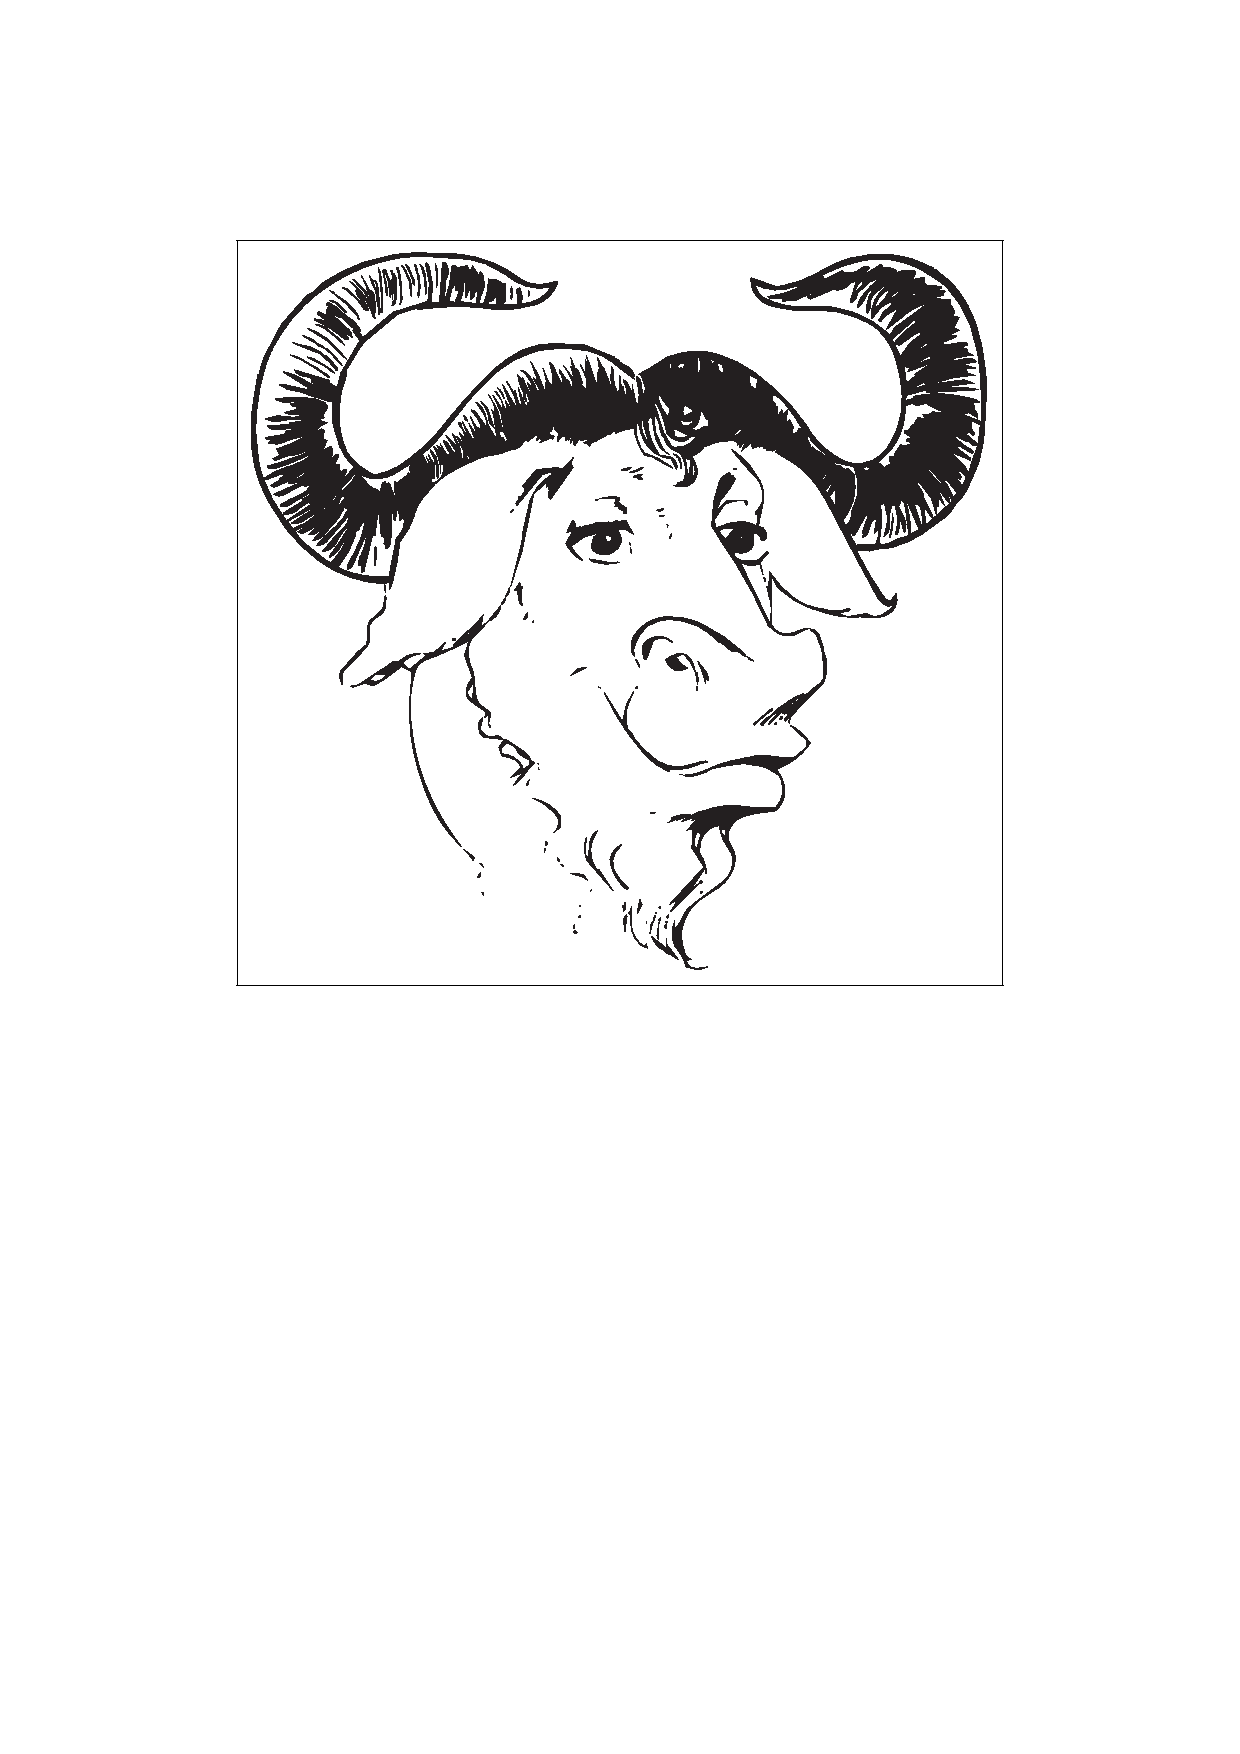
\includegraphics[width=.3\linewidth]{frame-gnu}}
\end{center}

\begin{center}
 \fbox{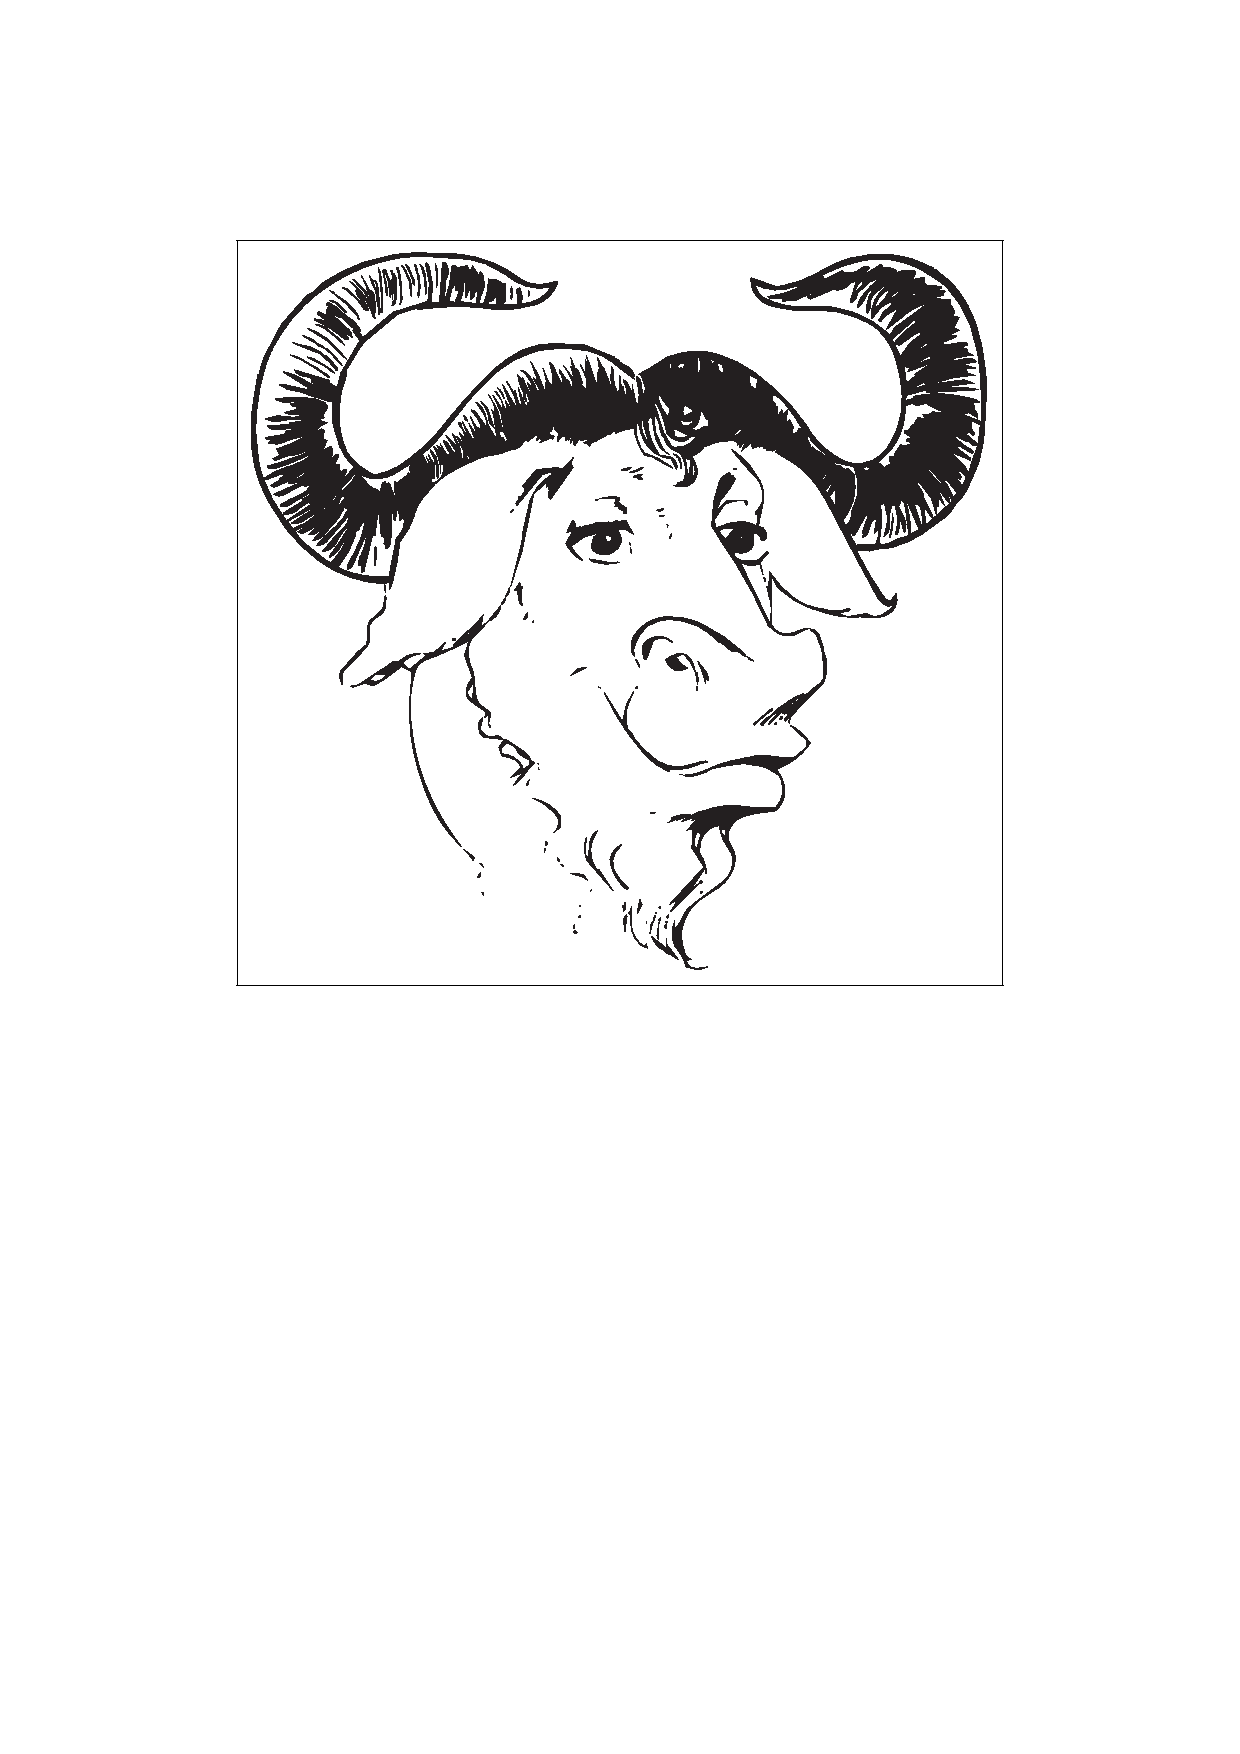
\includegraphics[width=.3\linewidth,trim=40 40 40 40]{frame-gnu}}
\end{center}

\begin{center}
 \fbox{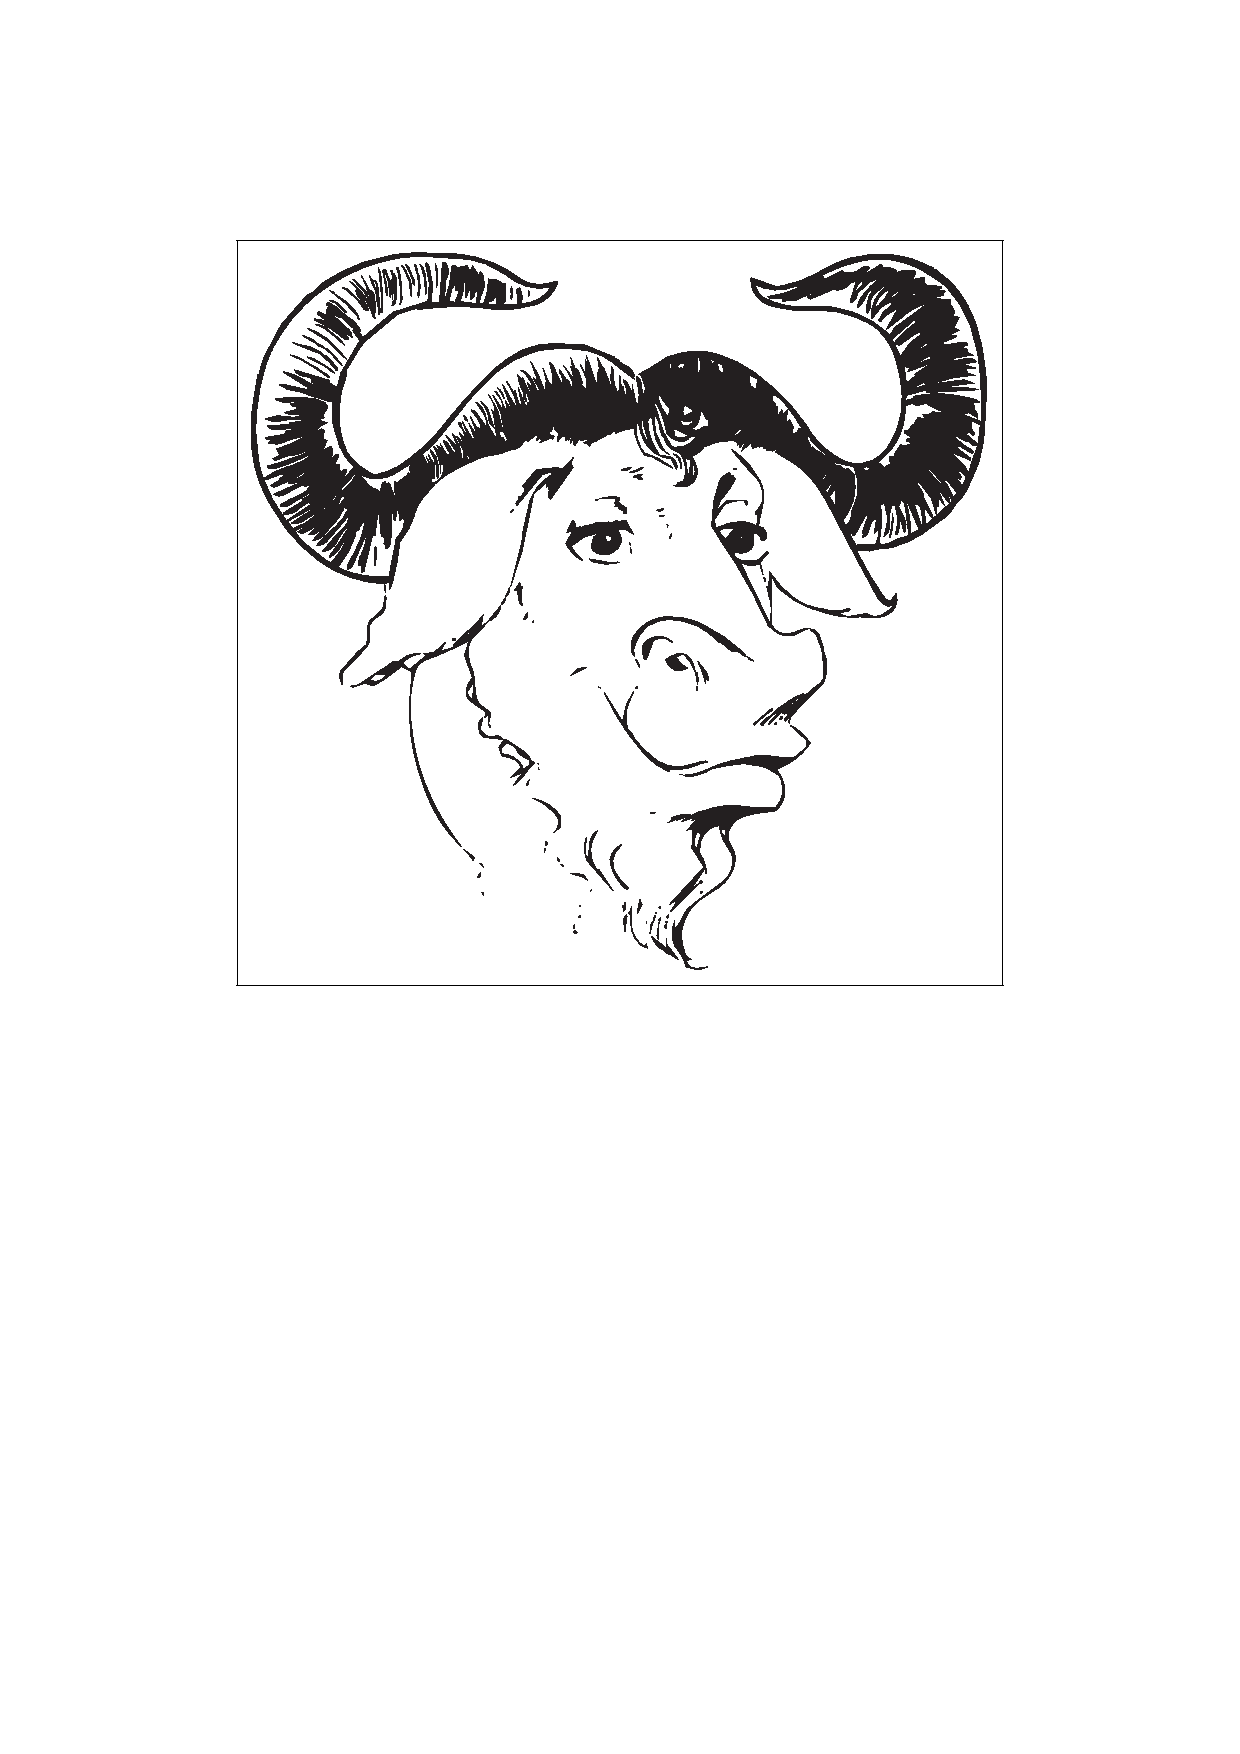
\includegraphics[width=.3\linewidth,clip,trim=40 40 40 40]{frame-gnu}}
\end{center}

\begin{center}
 \fbox{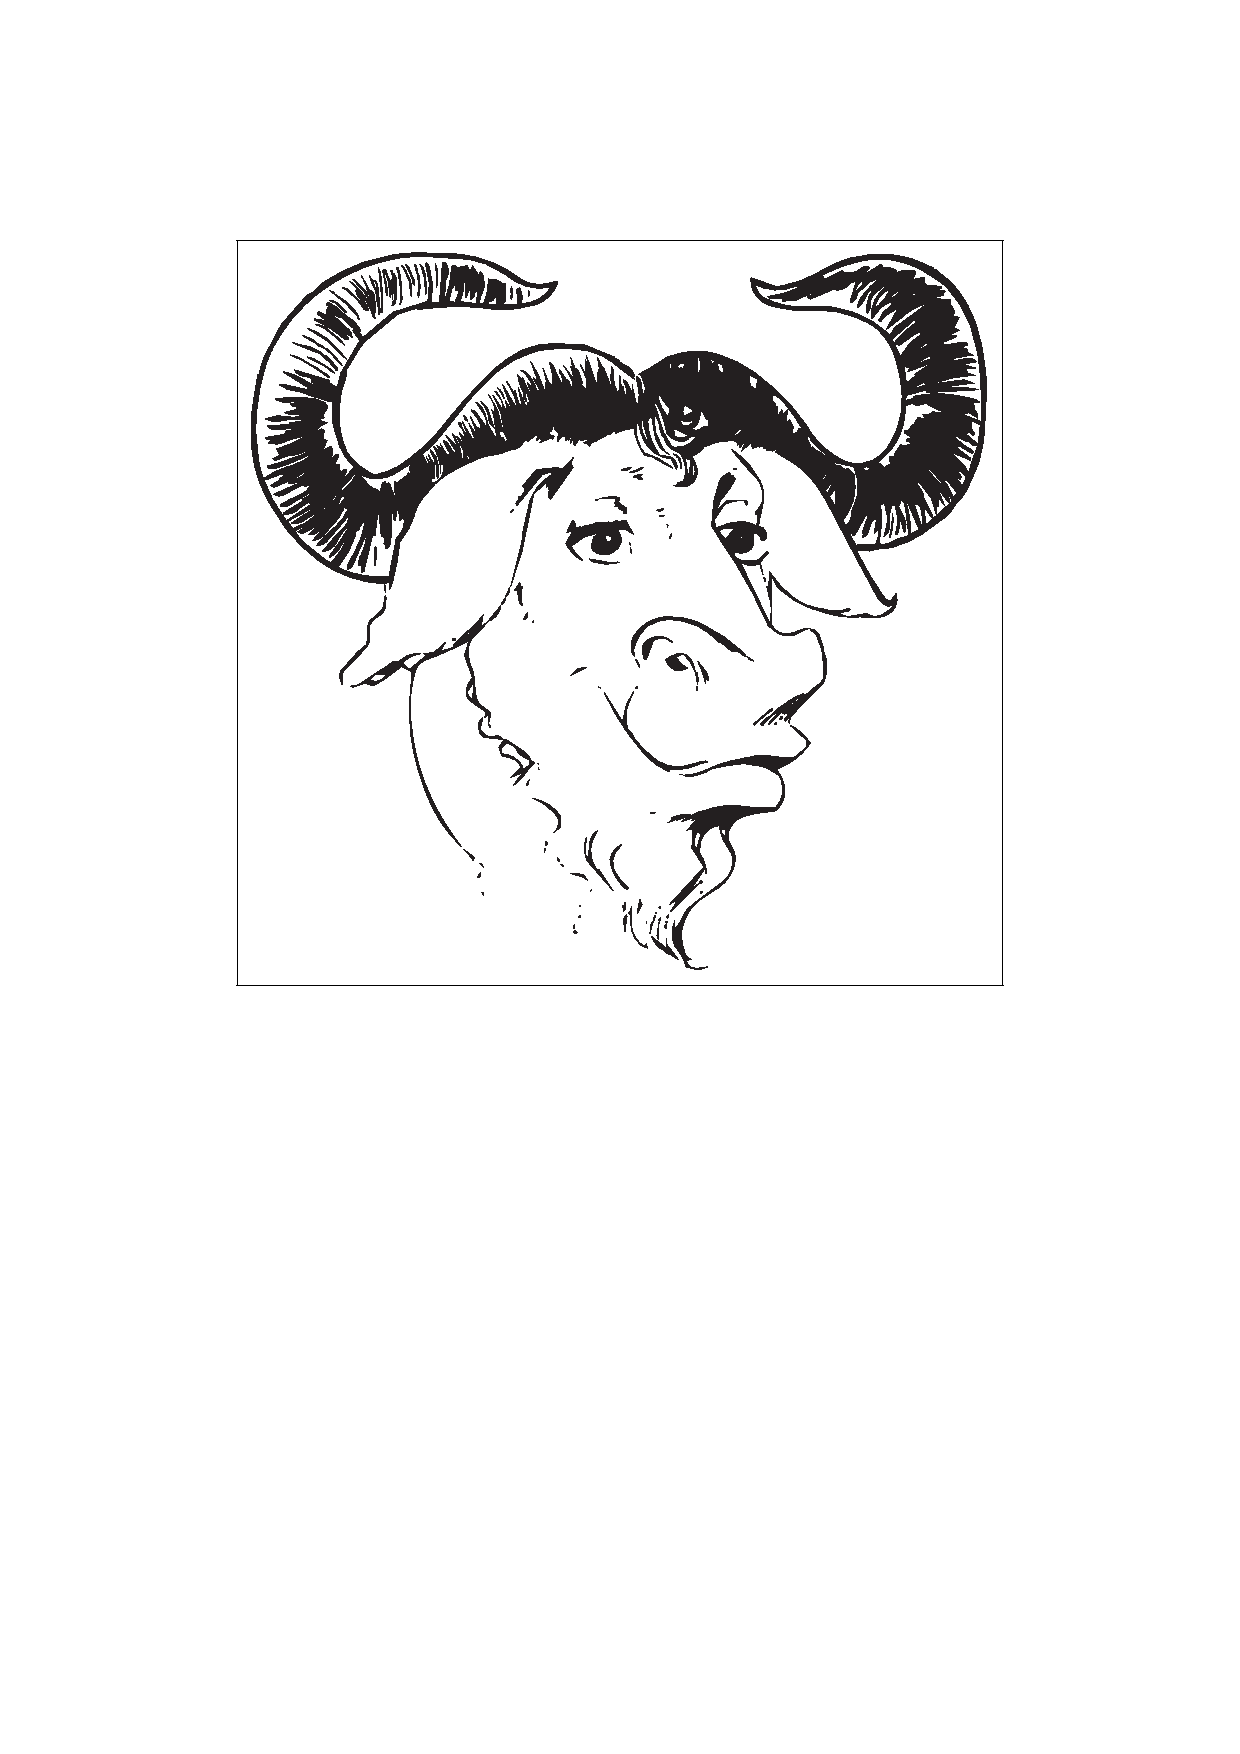
\includegraphics[width=.3\linewidth,clip,viewport=131 304 459 548]{frame-gnu}}
\end{center}

\begin{center}
 \fbox{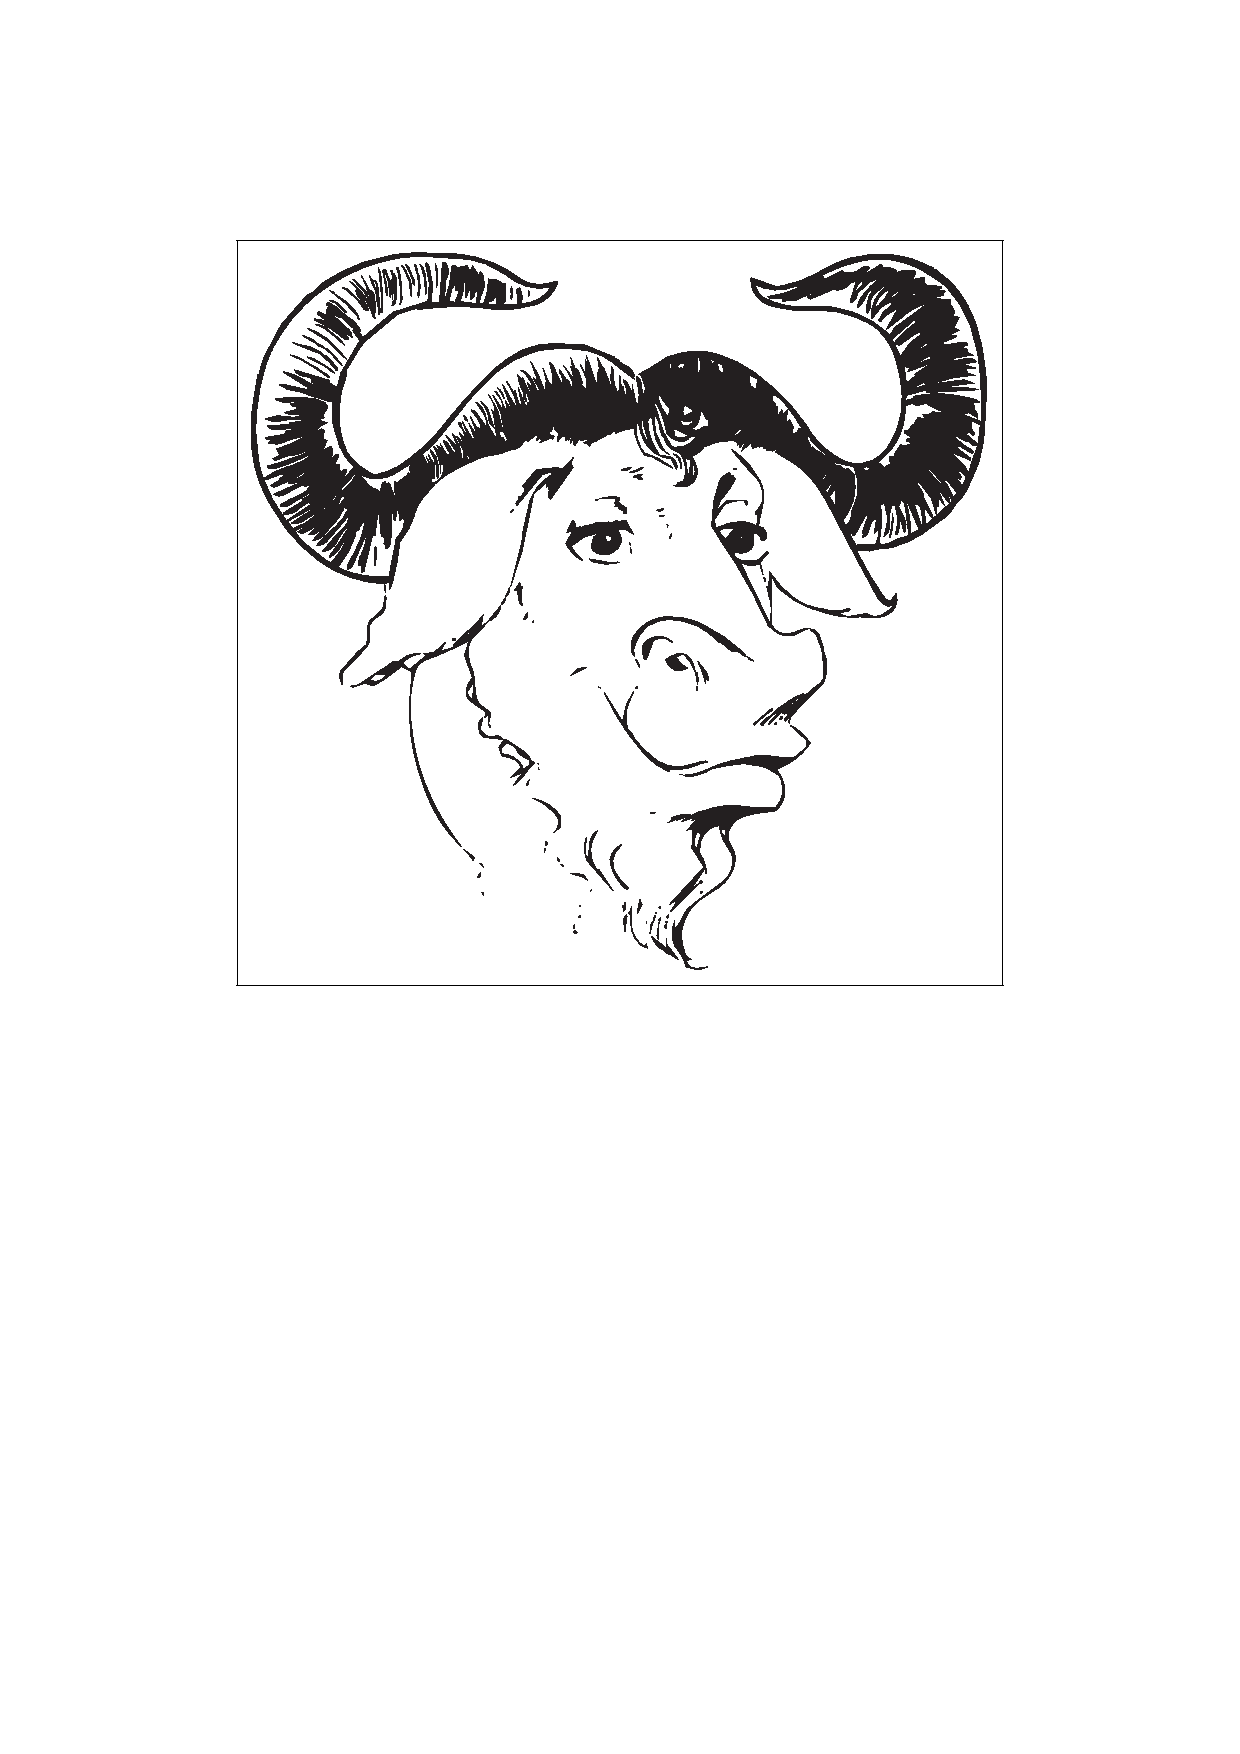
\includegraphics[width=.3\linewidth,angle=30]{frame-gnu}}
\end{center}

\begin{center}
 \fbox{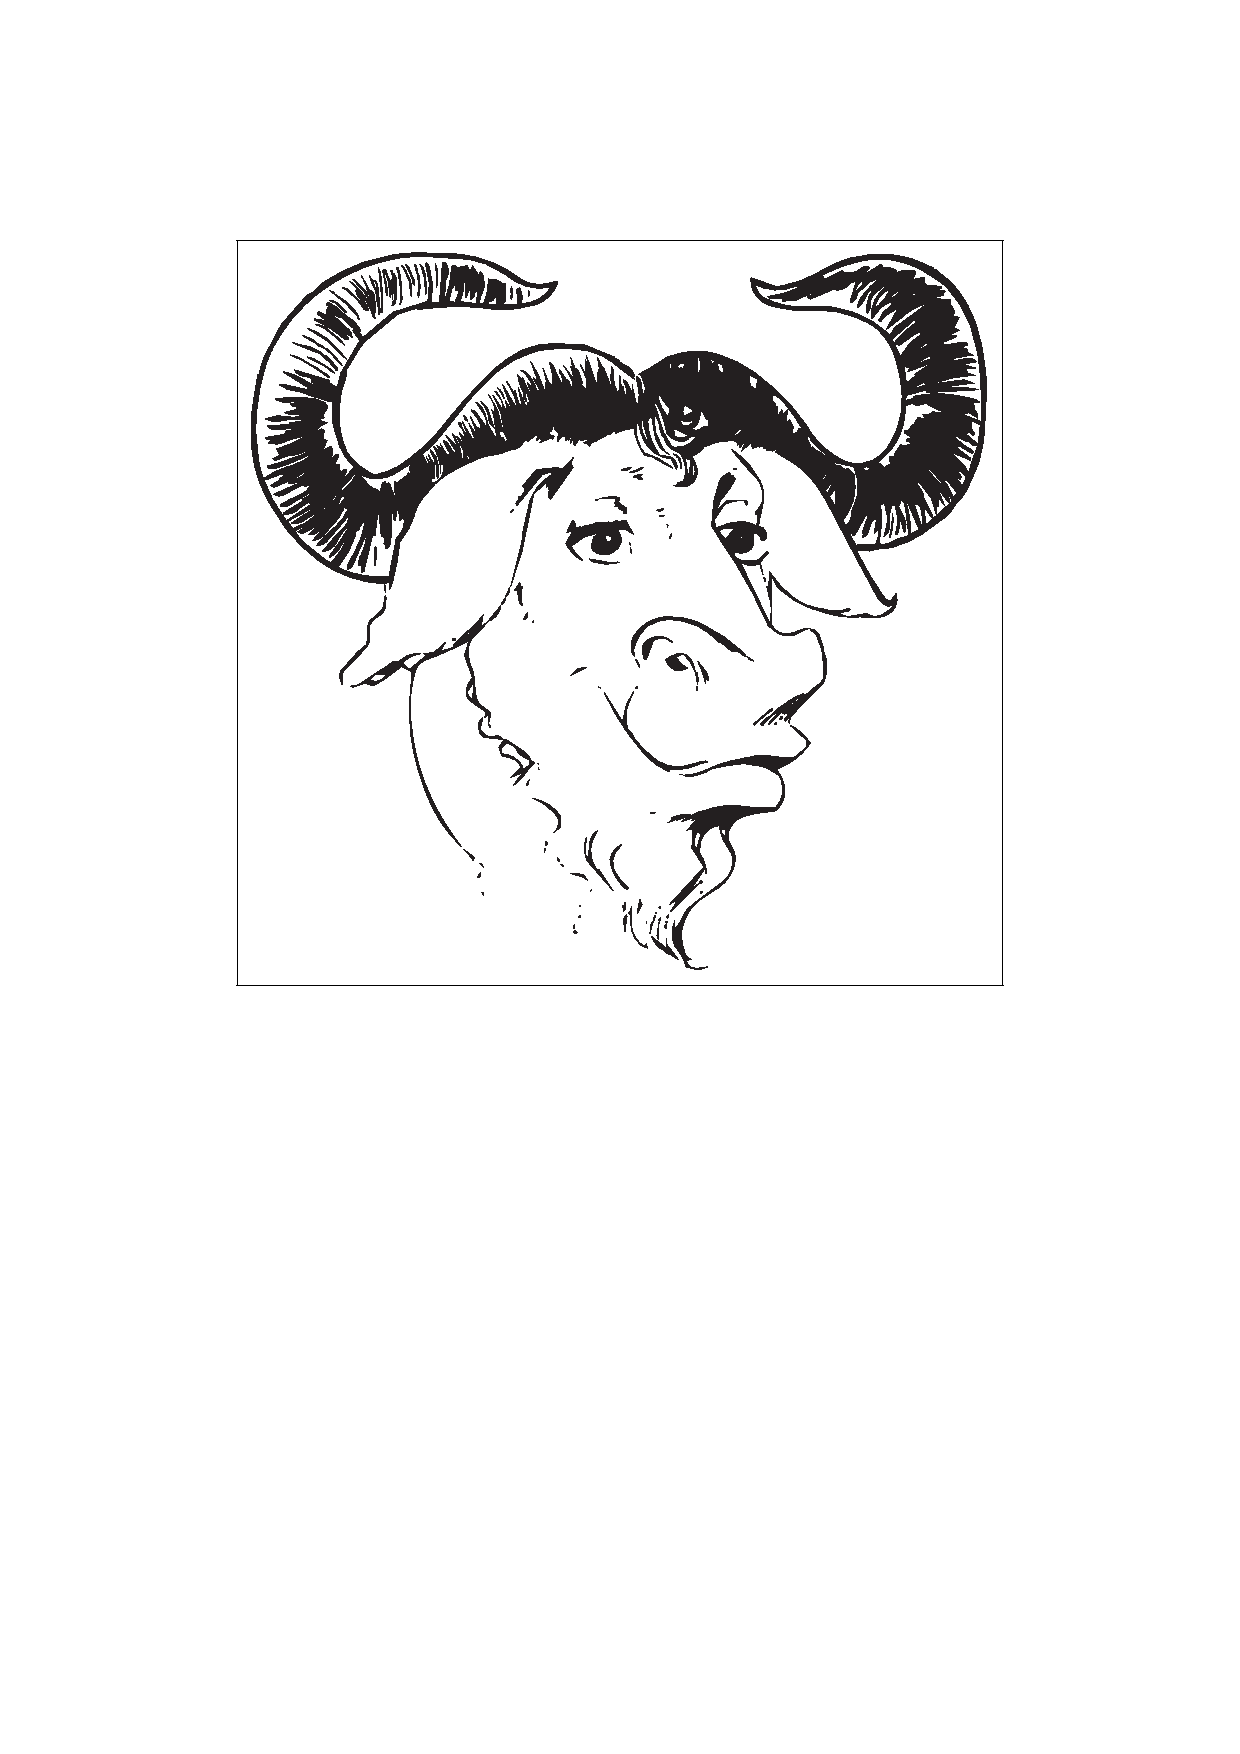
\includegraphics[width=.3\linewidth,angle=45,origin=tr]{frame-gnu}}
\end{center}


\subsection{図表を1段分の幅で張り込む}

2段組みにすると図表は用紙の文章幅 \C{textwidth}で
はなく1段分の幅 \C{columnwidth}で張り込む事に
なります.また以下の二つの環境が使えます.
\begin{usage}
table*環境
figure*環境 
\end{usage}
%\begin{Syntax}
%\Env{table*} 環境 \\
%\Env{figure*} 環境
%\end{Syntax}
\env{table}環境や\env{figure}環境にアスタリスクを付けると
その環境を1段分の幅でページの下部か上部に配置
しようとします.

\subsection{標準的に文章幅で画像を張り込む}

文書中の全ての図を文章幅で貼付ける
\verb|\setkeys{Gin}{width=\linewidth}|

\verb|\includegraphics[width=5cm]{file.pdf}|

とした処理をするが,

\verb|\includegraphics{file.pdf}|

とするだけで

\verb|\includegraphics[width=\linewidth]{file.pdf}|

と同じ効果がある.


\section{各種プログラムからの張り込み}

dvipdfmxによって最終的にPDFに変換する事を前提に説明します.

% この辺はいらないでしょう.コマンドブックの中には
% \subsection{\MP}
% \subsection{PSTricks}

\section{他のプログラムによる描画}
広く使われている描画ツールを紹介します.
以下の描画ツールで作成した図などは
それぞれ指定された方法でデバイスドライバが
適切に解釈できる状態になければなりません.


\subsection{グラフの描画}\seclab{gnuplot}
{\LaTeX}にグラフを挿入するには様々な方法が
あります.Windowsの方でならば{Excel}で作成した
グラフをEPSで保存し,それを\textsf{graphicx}パ
ッケージで読み込むという方法\pp{\secref{picture:program}参照}があります.
巷の表計算ソフトなんて使いたくない方は
\Person{Thomas}{Williams}と\Person{Colin}{Kelley}らによる
{Gnuplot}を使うと良いでしょう.{gnuplot}
はバージョン3.7に関しては\Hito{山賀}{正人}が,バージョ
ン3.8に関しては\Hito{尾田}{晃}がプログラムの日本語化を
されています.また{gnuplot}のマニュアルに
関しても\Hito{竹野}{茂治}らによって行われています\footnote{\webGplotman}.

\Z{制御系}では{SciLab}というのがあります.
マニュアルが\Hito{大野}{修一}らによって日本語化されています\footnote{\webScilabman}.

\Person{John}{Eaton}らによる{Octave}というのもあります
ので調べてみてください.



\subsection{Illustratorから図を張り込む}
何ら変換の必要はありません.

\subsection{Gnuplotから図を張り込む}
1. EPS -> PDF writer
2. {epic,eepic,amssymb} dashed rotated

\subsection{Microsoft Excel/OpenOffice.org Calcから図を張り込む}
1. PDF writer(クセロPDF) -> includegraphics 

\subsection{AutoCADから図を張り込む}

\subsection{ChemDrawから図を張り込む}

\subsection{ArcInfoから図を張り込む}

\subsection{SPSSから図を張り込む}

\subsection{Mathematicaから図を張り込む}

\subsection{xfigから図を張り込む}

\subsection{Octaveから図を張り込む}

\subsection{Scilabから図を張り込む}

\subsection{MatLabから図を張り込む}

\subsection{Rから図を張り込む}

\subsection{Tgifから図を張り込む}

\subsection{ngraphから図を張り込む}

\subsection{ありゃま,どったの?}

\begin{intext}
\documentclass[dvipdfm,dvipdfmx]{jsarticle}
\usepackage{epic,eepic,pict2e}% dvipdfm
\usepackage{geometry}% dvipdfm
\usepackage{hyperref}% dvipdfm
\usepackage{color,graphicx}% dvipdfmx
\end{intext}

\subsection{overpic}

package option
-percent [default]
-permil
-abs

graphicx, epic 必須

grid
tics
unit

% picture 環境と同じ, picture 環境の説明ないけど
\begin{usage}
\begin{overpic}[]{}
 
\end{overpic}
\end{usage}
